\documentclass[report]{jsbook}
\usepackage{amsthm,amsmath,amssymb,listings,ascmac,jlisting,docmute}
\usepackage[dvipdfmx]{graphicx}
% \usepackage[dviout]{graphicx}

\lstset{%
  language={C},
  basicstyle={\small},%
  identifierstyle={\small},%
  commentstyle={\small\itshape},%
  keywordstyle={\small\bfseries},%
  ndkeywordstyle={\small},%
  stringstyle={\small\ttfamily},
  frame={tb},
  breaklines=true,
  columns=[l]{fullflexible},%
  % numbers=left,%
  xrightmargin=0zw,%
  xleftmargin=3zw,%
  numberstyle={\scriptsize},%
  stepnumber=1,
  numbersep=1zw,%
  lineskip=-0.5ex%
}

\makeatletter
\long\def\@makecaption#1#2{{\small
  \advance\leftskip .0628\linewidth
  \advance\rightskip .0628\linewidth
  \vskip\abovecaptionskip
  \sbox\@tempboxa{#1\hskip1zw\relax #2}%
  \ifdim \wd\@tempboxa <\hsize \centering \fi
%  #1\hskip1zw\relax #2\par
  #1{\hskip1zw\relax}#2\par
  \vskip\belowcaptionskip}}
\makeatother


\title{近似的メッセージ伝搬法に基づく通信路とデータの同時推定}
\author{藤塚 拓実}
\date{\today}

\begin{document}
\maketitle
% 目次の表示
\tableofcontents
\newpage
% \chapter{概要}
今日,2020年までに,第5世代移動通信システム(5G)の国内での実用化に向けて,各研究機関,企業,大学が様々な研究・実験を実施している.

5Gの中心的技術として,大規模MIMOがある.大規模MIMOとは,基地局のアンテナを大量に保有することで,無線通信のスループットの向上を図る通信技術である.

しかし,信号を復調する際,従来の計算方法では,アンテナ数の増加に伴い,爆発に計算量が増えてしまう.そこで,本研究では,大規模MIMOの実現に向けて,復調の新たな計算方法として,人工知能の分野で提案された,近似的メッセージ伝播法(AMP)を用いてシミュレーションを行った.
\chapter{はじめに}
\section{研究背景}
2020年東京オリンピック・パラリンピック大会に向けて,日本国内の情報通信基盤(ICT)を飛躍的に向上させる戦略が,総務省を中心として活発になっている.その戦略の一つとして,第5世代移動通信システム(以下「5G」)の実現がある.\cite{soumu_suzuki}

近年スマートフォンのような高機能端末が一般層へ広く普及したことを起爆剤として,M2MやIoTが拡大していくことが予想されている.そのため,現行の4G/LTEよりもさらに,超高速・大容量のモバイル通信ネットワークとして,5Gの実現が求められる\cite{suyama}.

\section{大規模MIMO(Massive MIMO)}
5Gの中心的役割を担う技術が,大規模MIMO(massive MIMO)である.MIMO( Multiple Input Multiple Output)とは,送受信側が複数のアンテナを持ち合わせ持つことにより,データレート増加,ダイバーシチによる特性改善を図ることができるものである\cite{goldsmith}.4G/LTEで既に使用されているMIMOでは,基地局(受信側)のアンテナは2,4,8本程度しか持ち合わせていないが,大規模MIMOは,基地局のアンテナを100本以上まで増やし,同じ基地局を利用するユーザも100人規模までいることを仮定することで,多入力,多出力のシステムを想定している.図\ref{fig:mimo}に概念図を示す.
\begin{figure}[htbp]
  \begin{center}
    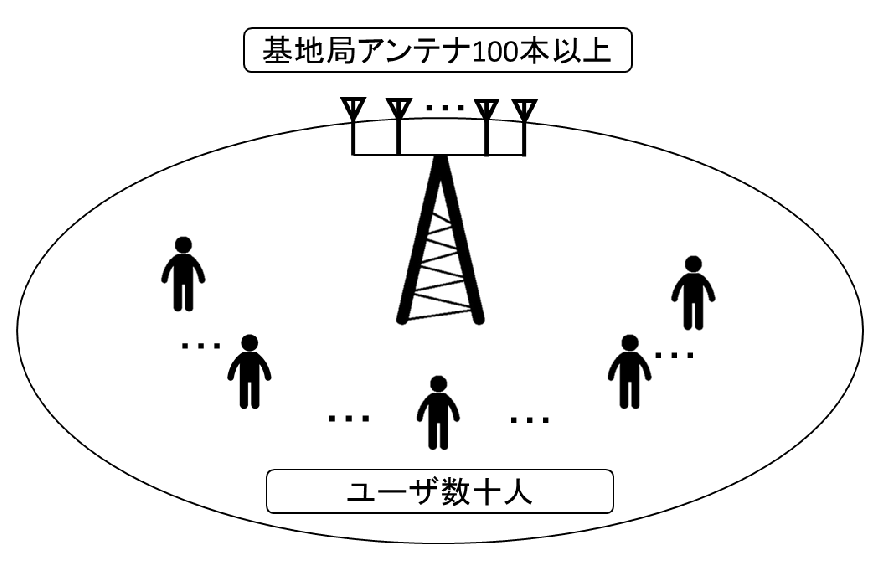
\includegraphics[clip,width=10.0cm]{./mimo.eps}
    \caption{大規模MIMOの概念図}
    \label{fig:mimo}
  \end{center}
\end{figure}


本研究では,大規模MIMOシステムの実用化に向けて,基地局側において,ユーザから送信された信号,また,その通信路について推定する.

\section{研究目的}
大規模MIMOでは,100本以上の基地局のアンテナの受信情報を効率的に演算し,送信信号を復調する必要がある.実際の大規模MIMOシステムでは,基地局間干渉が発生するため,受信側の基地局では,別の基地局のユーザからの干渉を受けることになる.本研究では,基地局間干渉を考慮したうえで,基地局側が信号を復調する際,別の基地局の信号と自身の基地局の信号を分離できるような計算方法を確立することを目的とする.

\section{研究内容}
大規模MIMOの復調の計算方法として,近似的メッセージ伝搬法(Approximate Message Passing 以下「AMP」)を用いる.AMPは,人口知能分野で提案された確率伝播法(Belief Propagation BP)を基礎として発展した統計学的手法であり.もともとは,圧縮センシングの分野で提案された手法である\cite{Donoho}.

AMPアルゴリズムを用いて,二つの行列の積の情報より,元の二つの行列を推定する体系的な理論は,参考文献\cite{kabashima}の著者である樺島祥介氏らによって考案された.参考文献\cite{kabashima}では,あくまで,体系的な理論を説明し,広い範囲において適応できるシミュレーションにとどまっているが,本研究では大規模MIMOの基地局間干渉がある事象に的を絞った.具体的には,図\ref{fig:matrix}に示すように,推定する二つの行列を通信路と送信データとして,二つの行列の積の結果に白色雑音を足したものを大規模MIMOのアンテナが受け取る受信信号として,受信信号より通信路と送信データを推定する.
\begin{figure}[htbp]
  \begin{center}
    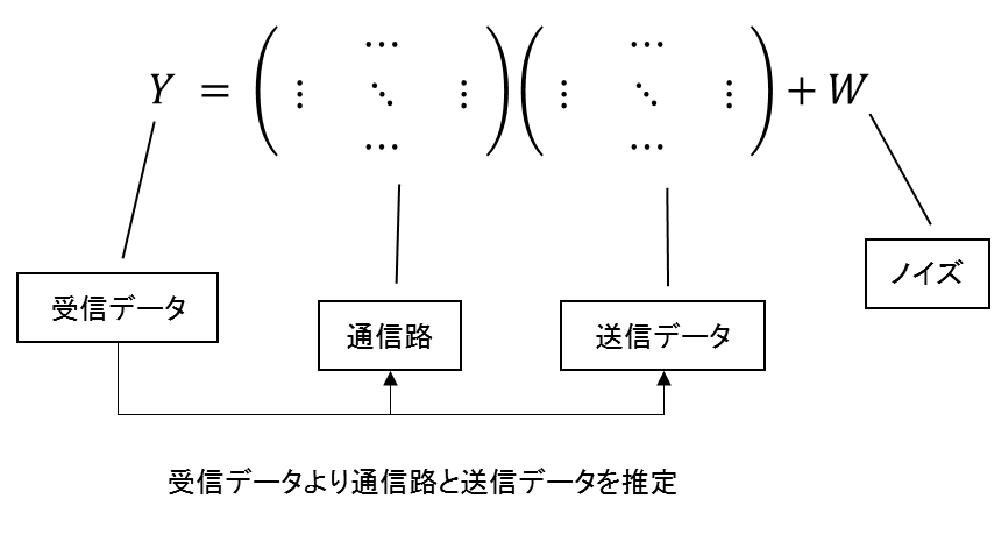
\includegraphics[clip,width=10.0cm]{./matrix.eps}
    \caption{想定しているシステムの行列}
    \label{fig:matrix}
  \end{center}
\end{figure}


\section{論文構成}
\chapter{提案手法}
\section{アップリンクマルチユーザMIMO}
本研究は,複数ユーザが基地局に情報を送るアップリンクを想定して研究を行った.ユーザ数を$K$,受信アンテナ数を$N$とし,ユーザは単一の送信アンテナを持つことを想定する.また,簡単のため,フェージング係数が観測時間$T$の間一定であるブロックフェージング通信路を仮定する.受信信号$\boldsymbol{Y}\in\mathbb{C}^{N\times T}$は式(\ref{eq:ReceiveSignal})にて与えられる.
\begin{equation} 
	\label{eq:ReceiveSignal}
	\boldsymbol{Y} = \frac{1}{\sqrt{N}}\boldsymbol{HX+W}.
\end{equation}
$1/\sqrt{N}$は正規化定数であり,アンテナ数の上昇による電力の上昇を抑える.$\boldsymbol{X}\in\mathbb{C}^{K\times T}$は全ユーザの送信信号であり,$\boldsymbol{H}\in\mathbb{C}^{N\times K}$はすべてのユーザとアンテナ間のフェージング係数である.ここで,$\boldsymbol{H}$に関して,すべての行列成分は,互いに独立で同一の分布(independent and identically distribution : i.i.d)のレイリーフェージングに従うと仮定する.具体的には,それぞれが独立した円対称複素ガウス雑音(circularly symmetric complex Gaussian : CSCG)であり,分散は1とした.また,$\boldsymbol{W}\in\mathbb{C}^{N\times T}$は受信時に生じる雑音のことであり,それぞれが独立した円対称複素ガウス雑音で,分散は定数$N_0$とした.

ここで,基地局間干渉のため,ユーザーを二つのグループに分ける.一方のグループは自分の基地局のエリアに存在するユーザで,$K/2$人で構成され,残る$K/2$人のユーザは別の基地局のエリアのユーザであり,自分の基地局の信号に干渉してくる.これを踏まえ,$\boldsymbol{X}$を式(\ref{eq:SendSignal})のように定義する.
\begin{equation} 
	\label{eq:SendSignal}
	\boldsymbol{X} =  \left(
		\begin{array}{cccc}
			\boldsymbol{X}_{11} &\boldsymbol{X}_{12} &\boldsymbol{P}\\
			\boldsymbol{P} &\boldsymbol{X}_{21} &\boldsymbol{X}_{22}.
		\end{array}
	\right)
\end{equation}
$\boldsymbol{P}$は$K/2\times T_{p}$のパイロット行列であり,基地局側にとってこの信号は既知である.$\boldsymbol{X}$の行方向は観測時間$T$であるので,$\boldsymbol{P}$の送信時間の違いによって,行列(\ref{eq:SendSignal})は上半分と下半分で基地局を分けている.また,$\boldsymbol{X}$信号はそれぞれ,式(\ref{eq:QPSK})のような電力1のQPSK信号である.電力1というのは,ユーザの長期的な平均電力とする.
\begin{equation} 
	\label{eq:QPSK}
	x_{kt} = \{u+jv:u,v=\pm\sqrt{1/2}\}.
\end{equation}

\section{通信路推定とデータ推定}
受信側で推定するデータを$\hat{\boldsymbol{X}}$として,ここでは,推定するデータは事後平均推定
\begin{equation} 
	\label{eq:PosterorMean}
	\hat{\boldsymbol{X}}=\mathbb{E}[\boldsymbol{X}|\boldsymbol{Y},\boldsymbol{P}]
\end{equation}	
を目標とする.しかし,大規模MIMOシステムでは,式(\ref{eq:PosterorMean})は$K,N,T$の上昇に伴い,指数関数的に上昇するため現実的な時間で解くことは,不可能である.そこで,AMPアルゴリズムを用いる.詳しい式の導出は,\ref{sec:AMP}章に譲る.AMPアルゴリズムを使う条件として,$N,K,T,Tp$が無限大に近く,$\alpha=K/N$,$\beta=T/N$,$\tau=T_{p}/T$が一定で保たれる必要がある.AMPアルゴリズムでは,表\ref{tb:Message}で示される8つのメッセージをそれぞれ交換することで推定を行っていく.初期値として,パイロット信号が入っている$(k,t) \in \{1,...,K/2\}\times \{T-T_{p}+1,...,T\}$もしくは$(k,t) \in \{K/2+1,...,K\}\times \{1,...,T_{P}\}$のとき,$\hat{x}_{kt}=x_{kt}$,$\xi_{kt}=0$となり,パイロット信号が入っていない,それ以外の成分は$\hat{x}_{kt}=0$,$\xi_{kt}=1$とした.また,他の要素は,$\hat{h}_{nk}=0$,$\eta_{nt}=1$,$\overline{I}_{nt}=0$,$\zeta_{nt}=0$とした.
\begin{table}[htb]
	\begin{center}
		\caption{AMPアルゴリズムで使用されるメッセージ \label{tb:Message}}
		\begin{tabular}{|c|c|} \hline
			$\hat{x}_{kt}$ & $x_{kt}$の事後平均 \\ \hline
			$\xi_{kt}$ & $x_{kt}$の事後分散 \\ \hline
			$\overline{x}_{kt}$ & $x_{kt}$の外部平均 \\ \hline
			$\overline{\xi}_{kt}$ & $x_{kt}$の外部分散 \\ \hline\hline
			$\hat{h}_{nk}$ & $h_{nk}$の事後平均 \\ \hline
			$\eta_{nk}$ & $h_{nk}$の事後分散 \\ \hline\hline
			$\overline{I}_{nt}$ & $y_{nt}$の干渉の平均 \\ \hline
			$\zeta_{nt}$ & $y_{nt}$の干渉の分散 \\ \hline
		\end{tabular}
	\end{center}
\end{table}

ここで,各メッセージを計算するための定義式を記す.まず,干渉を差し引いた出力$z\in\mathbb{C}$は
\begin{equation} 
	\label{eq:z}
	z_{nt}=\frac{y_{nt}-\overline{I}_{nt}}{N_{0}+\zeta_{nt}}
\end{equation}
と定義する.$\Re[x_{kt}]$の軟判定関数として,以下のような関数を定義する.
\begin{equation} 
	\label{eq:fk}
	f_{k}(u;v)=\frac{1}{\sqrt{2}}
			\frac{e^{\sqrt{2}u/v}-e^{-\sqrt{2}u/v}}{e^{\sqrt{2}u/v}+e^{-\sqrt{2}u/v}}.
\end{equation}
複素関数$A_{kt}(z)$として,以下のような関数を定義する.
\begin{equation} 
	\label{eq:Akt}
	A_{kt}(z)=\Re[z]\frac{\partial f_{k}}{\partial u}(\Re[\overline{x}_{kt}];\overline{\xi}_{kt})+j\Im[z]\frac{\partial f_{k}}{\partial u}(\Im[\overline{x}_{kt}];\overline{\xi}_{kt}).
\end{equation}
データ推定に関わるメッセージの式を以下に示す.
\begin{equation} 
	\label{eq:x_h}
	\hat{x}_{kt}=f_{k}(\Re[\overline{x}_{kt}],\overline{\xi}_{kt})+jf_{k}(\Im[\overline{x}_{kt}],\overline{\xi}_{kt}),
\end{equation}
\begin{equation} 
	\label{eq:xi}
	\xi_{kt} = 1 - |\hat{x}_{kt}|^2,
\end{equation}
\begin{equation} 
	\label{eq:x_b}
	\overline{x}_{kt} = 
		\frac{\overline{\xi}_{kt}}{\sqrt{N}}
			\sum_{n=1}^{N}\hat{h}^{*}_{nk}z_{nt}
			+\left(
				1-\frac{\overline{\xi}_{kt}}{N}\sum_{n=1}^{N}\eta_{nk}|z_{nt}|^2
			\right)
			\hat{x}_{kt},
\end{equation}
\begin{equation} 
	\label{eq:xi_b}
	\overline{\xi}_{kt}=
	\left(
		\frac{1}{N}
		\sum_{n=1}^{N}
			\frac
			{|\hat{h}_{nk}|^{2}}
			{N_{0}+\zeta_{nt}}
	\right)^{-1}.
\end{equation}
通信路推定に関するメッセージの式を示す.
\begin{equation}
	\label{eq:h_h}
	\hat{h}_{nk}=
	\frac
		{\eta_{nk}}
		{\sqrt{N}}
	\sum_{t=1}^{T}
		\hat{x}^{*}_{kt}z_{nt}
	+
	\left(
		1-\eta_{nk}
	\right)
	\hat{h}_{nk}
	-
	\frac
		{\eta_{nk}}
		{N}
	\sum_{t=1}^{T}
		\overline{\xi}_{kt}
		A^{*}_{kt}
		\left(
			\hat{h}_{nk}^{*}
			z_{nt}
		\right)
		z_{nt},	
\end{equation}
\begin{equation}
	\label{eq:eta}
	\eta_{nk}=
	\left(
		1+
		\frac{1}{N}
		\sum^{T}_{t=1}
			\frac
			{|\hat{x}_{kt}|^{2}}
			{N_{0}+\zeta_{nt}}
	\right)^{-1}.
\end{equation}
最後に,干渉に関するメッセージの式を示す.
\begin{equation}
	\label{eq:I_b}
	\overline{I}_{nt}=
		\frac{1}{\sqrt{N}}
		\sum_{k=1}^{K}
			\hat{h}_{nk}\hat{x}_{kt}
		-
		\frac{1}{N}
		\sum^{K}_{k=1}
			\overline{\xi}_{kt}
			A_{kt}
			\left(
				\hat{h}_{nk}^{*}
				z_{nt}
			\right)
			\hat{h}_{nk}
		-
		\frac{1}{N}
		\sum^{K}_{k=1}
			\eta_{nk}
			|\hat{x}_{kt}|^{2}
			z_{nt},
\end{equation}
\begin{equation}
	\label{eq:zeta}
	\zeta_{nt}=
		\sum_{k=1}^{K}
			\left(
				\eta_{nk}\xi_{kt}
				+
				\eta_{nk}|\hat{x}_{kt}|^{2}
				+
				|\hat{h}_{nk}|^{2}\xi_{kt}
			\right)
\end{equation}
AMPアルゴリズムでは,式(\ref{eq:x_h})-(\ref{eq:zeta})を計算することで,通信路とデータを同時推定する.
\chapter{導出}
\section{近似的確率伝搬法 (Belief Propagetion BP)}
\section{近似的メッセージ伝播法 (Approximate Message Passing AMP)}

\newpage
  \begin{thebibliography}{10}
    \bibitem{soumu_suzuki}
    鈴木 茂樹, ``2020年に向けた情報通信基盤整備の戦略,'', 2014, 2016年11月22日閲覧 \\ {https://www.nic.ad.jp/ja/materials/iw/2014/proceedings/d2/d2-suzuki.pdf}
    \bibitem{suyama}
    須山 聡, シン キユン, 小原 辰徳, 角 誠, 中島 光雅, 奥村 幸彦, ``高周波数帯を用いた超高速MassiveMIMO伝送の基本特性'', 信学技報, 2014年3月.
    \bibitem{goldsmith}
    Abdrea Goldsmith, ``Wireless Communication'', Cambridge University Press, 2005, (訳)小林 岳彦・ 岩切 直彦・大坐畠 智・幸谷 智・高橋 賢・森 香津夫・山嵜 彰一郎, ``ゴールドスミス ワイヤレス通信工学 基礎理論からMIMO,OFDM,アドホックネットワークまで'', 丸善株式会社, , p.297, 2007
    \bibitem{Donoho}
    D. L. Donoho, A. Maleki, and A. Montanari, “Message-passing algorithms for compressed sensing,” Proc. Nat. Acad. Sci. USA, 2009. 
    \bibitem{kabashima}
    Yoshiyuki Kabashima, Florent Krzakala, Marc Mézard, Ayaka Sakata, and Lenka Zdeborová, ``Phase Transitions and Sample Complexity in Bayes-Optimal Matrix Factorization '' , IEEE TRANSACTIONS ON INFORMATION THEORY, VOL. 62, NO. 7, 2016

  \end{thebibliography}
\end{document}

